\chapter{BUY and SELL in Chadic languages} \label{ch:buysell}

Like the preceding chapter, this chapter focuses on a particular functional domain in which many Chadic languages employ directional extensions. Chapter \ref{ch:CAM} covers the domain of directed caused accompanied motion. This chapter covers the domain of commercial transactions, specifically buying and selling events. 

The ancestors of speakers of Chadic languages entered the Sahel region around 6,000 years ago \citep[71]{maceachernUnderstandingDistributionsChadic2018a}. They developed their languages in a context where commerce was predominantly done through trading goods. At some point in the last few millennia, the use of currency became the dominant mode of commerce. Speakers of Chadic languages began adapting to a new distinction: framing a commercial exchange in terms of which party gives or receives money (BUY or SELL).

Various strategies are used to make the distinction between buying and selling: the meaning of an existing verb may be extended, a verb may be borrowed from another language, or existing morphosyntactic forms can be co-opted to mark the distinction. The particular means used vary within each branch of Chadic languages in a way that does not align with genetic subgroupings. Yet, in this diversity, there is a remarkably consistent pattern of nearly always using an innovative form to overtly mark the SELL meaning, rather than BUY. This asymmetry reflects a goal-oriented bias in the expression of transfer of possession events \citep{lakustaStartingEndImportance2005,georgakopoulosFramingDifferenceSources2015}.

This chapter presents a study of the distribution of the various grammatical strategies that evolved for expressing these currency-related concepts in the grammars of 85 Chadic languages. Section \ref{sec:distinguishing} gives an overview of how many languages use each means of distinguish BUY and SELL. Cases of borrowed verbs or semantic shift to express SELL are discussed in Section \ref{sec:borrow}. Selling events can also be marked by verbal morphology (Section \ref{sec:SELLmorph}) or syntactic means (Section \ref{sec:SELLsyntax}). The rare instances of forms overtly marked for a BUY meaning are discussed in Section \ref{sec:BUYmorph}. Finally, Section \ref{sec:BUYsummary} provides a summary and discussion of the implications of this analysis.

\section{Distinguishing BUY and SELL} \label{sec:distinguishing}

Buying and selling events entail the exchange of money for goods. In a buying framing of the event (BUY), the person receiving the goods and giving money is the subject and the other participant is not necessarily a core argument, e.g., \textit{I bought a new car} (\textit{from my neighbor}). In a selling framing of the event (SELL), the person giving the goods and receiving the money is the subject and the buyer is not necessarily a core argument, e.g., \textit{I sold my car} (\textit{to my neighbor}). The distinction between BUY and SELL is an example that has been used by several linguists to illustrate how the same real world event can be construed differently by linguistic structures. \citet[25--26]{fillmoreTopicsLexicalSemantics1977} uses BUY and SELL to illustrate how different verbs can provide alternative ``perspectives'' on the same ``scene''.  \citet[77]{talmyCognitiveSemantics2000} refers to the choice between BUY and SELL as ``mapping of attention''. \citet[81]{geeraerts2000salience} refers to it as ``variational salience''. 

Many Chadic languages have a verb root that is ambivalent; it can be used for either BUY or SELL framing of a commercial transaction. For example, in \hyperref[dang]{Dangla}, the verb root \textit{gídy} (glossed `trade' in the original) occurs in the context of describing both BUY events (the subject is the buyer), as in (\ref{ex:dang0}), as well as SELL events, (the subject is the seller), as in (\ref{ex:dang1}). 

\ea\label{ex:dang0}
\langinfo{\hyperref[dang]{Dangla} verb \textit{gídy} `buy/sell' translated as BUY}{}{\cite[140]{shayGrammarEastDangla1999}} \\
\gll ŋu gidiy bèrka \\
3\gl{pl} buy/sell.\gl{pst} cow \\
\glt `They bought a cow.'

\ex\label{ex:dang1}
\langinfo{\hyperref[dang]{Dangla} verb \textit{gídy} `buy/sell' translated as SELL}{}{\cite[146]{shayGrammarEastDangla1999}} \\
\gll ŋa gidày-tʸa bèrka súgín-írá \\
3\gl{m} buy/sell.\gl{pst}-3\gl{f}.\gl{obj} cow market-\gl{loc} \\
\glt `He sold the cow at the market.'
\z

The label TRADE (in all capital letters) is used here for an unmodified verb root that can be used to express either BUY or SELL. In Dangla, the available data does not reveal any lexicalized or morphosyntactic mechanism for distinguishing BUY and SELL. This is the case for nine of the 85 Chadic languages in the sample. It may be that speakers rarely find themselves describing a context where there is ambiguity about the buyer and seller roles in a transaction, or such contexts may be so rare that non-grammaticalized means can be used, such as adding another phrase or clause to explicitly state who gave money and who received money in the transaction. It should be noted, however, there is limited documentation available for these nine languages, and so there is a strong possibility of a gap in the data.  

More commonly, languages with a TRADE verb root have a mechanism for distinguishing BUY and SELL. For example, the TRADE verb root \textit{pá} `buy/sell' in \hyperref[psik]{Psikye} is found in examples where it is translated `buy', as in (\ref{ex:psik28}), and also where it is translated `sell', as in (\ref{ex:psik29}). However, with the bushward suffix, as in (\ref{ex:psik25}), the verb can only express SELL.

\ea\label{ex:psik28}
\langinfo{\hyperref[psik]{Psikye} verb \textit{pá} `buy/sell'}{}{\cite[65]{smithKapsikiLanguage1969}} \\
\gll pa Hunter nde-ke ɗá cɛɗɛ ka-pa xá	\\
then Hunter give-\gl{vent} me money \gl{ipfv}-buy/sell millet \\
\glt `Then Hunter gave me money to buy millet.'

\ex\label{ex:psik29}
\langinfo{\hyperref[psik]{Psikye} verb \textit{pá} `buy/sell'}{}{\cite[60]{smithKapsikiLanguage1969}} \\
\gll pa xɛ́ vi-yi kweté wundú ka-pá nda ka xɛ́ 	\\
then 3\gl{pl} ??-put certain person \gl{ipfv}-buy/sell for ?? 3\gl{pl} \\
\glt `Then they put a certain person to sell (it) for them.'
\z 

\ea\label{ex:psik25}
\langinfo{\hyperref[psik]{Psikye} bushward form of \textit{pá} `buy/sell'}{}{\cite[114]{smithKapsikiLanguage1969}} \\
\gll 'a 'ya ké-pá-mte marure kwélékwelé	\\
\textsc{active} 1\gl{sg} \gl{ptcp}-buy/sell-\gl{bush} rice much \\
\glt `I sold a lot of rice.'
\z 

In Chadic languages, there are variety of means for distinguishing between BUY and SELL. \tabref{tab:BUYSELL} gives an overview of the how many languages have evidence of each of the strategies for distinguishing BUY and SELL. As seen in (\ref{ex:psik25}), one common strategy is to co-opt existing verbal morphology to modify a TRADE verb and designate the modified form as SELL. This is found in 29 of the 85 languages in the sample. Within this strategy, there is variation in which grammatical means are used to distinguish the meanings. The other common strategy, attested in 38 languages, is to incorporate a new verb root to make the distinction, either through borrowing or semantic shift. In this approach, the innovative verb root expresses SELL, and the meaning of an erstwhile TRADE verb may be restricted to only mean BUY.

Less commonly found means of making the distinction between BUY and SELL include the use of syntactic constructions with an adverbial or prepositional phrase (found in eight languages), and, in just four languages, the use of morphology to overtly mark a BUY event.

\begin{table}[H]
	\caption{Number of Chadic languages using each means for distinguishing BUY and SELL}
	\label{tab:BUYSELL}
	\begin{tabular}{l@{}rrrrr} % add l for every additional column or remove as necessary
		\lsptoprule
	{}	      &  West (26) &  Biu-M. (41) &  Masa (4) &  East (14) &  Total \\
	\midrule
No distinction       &     6 &            0 &     0 &     3 &      9 \\
%TRADE verb           &     9 &           12 &     0 &     7 &     28 \\
%BUY verb             &    17 &           28 &     4 &     7 &     56 \\
SELL verb            &     9 &           22 &     1 &     6 &     38 \\
SELL via syntax     &     3 &            2 &     1 &     2 &      8 \\
SELL via morphology &     8 &           16 &     2 &     3 &     29 \\
BUY via morphology  &     0 &            4 &     0 &     0 &      4 \\
		\lspbottomrule
	\end{tabular}
\end{table}

The geographic distribution of languages using various strategies for expressing SELL or BUY are shown in Figure \ref{fig:buysell}. The lack of clear geographical patterns suggest that there has not been a significant amount of contact or areal influence on the means for distinguishing BUY and SELL.

%see R code in file 'CAM map R code' 
\begin{sidewaysfigure}
	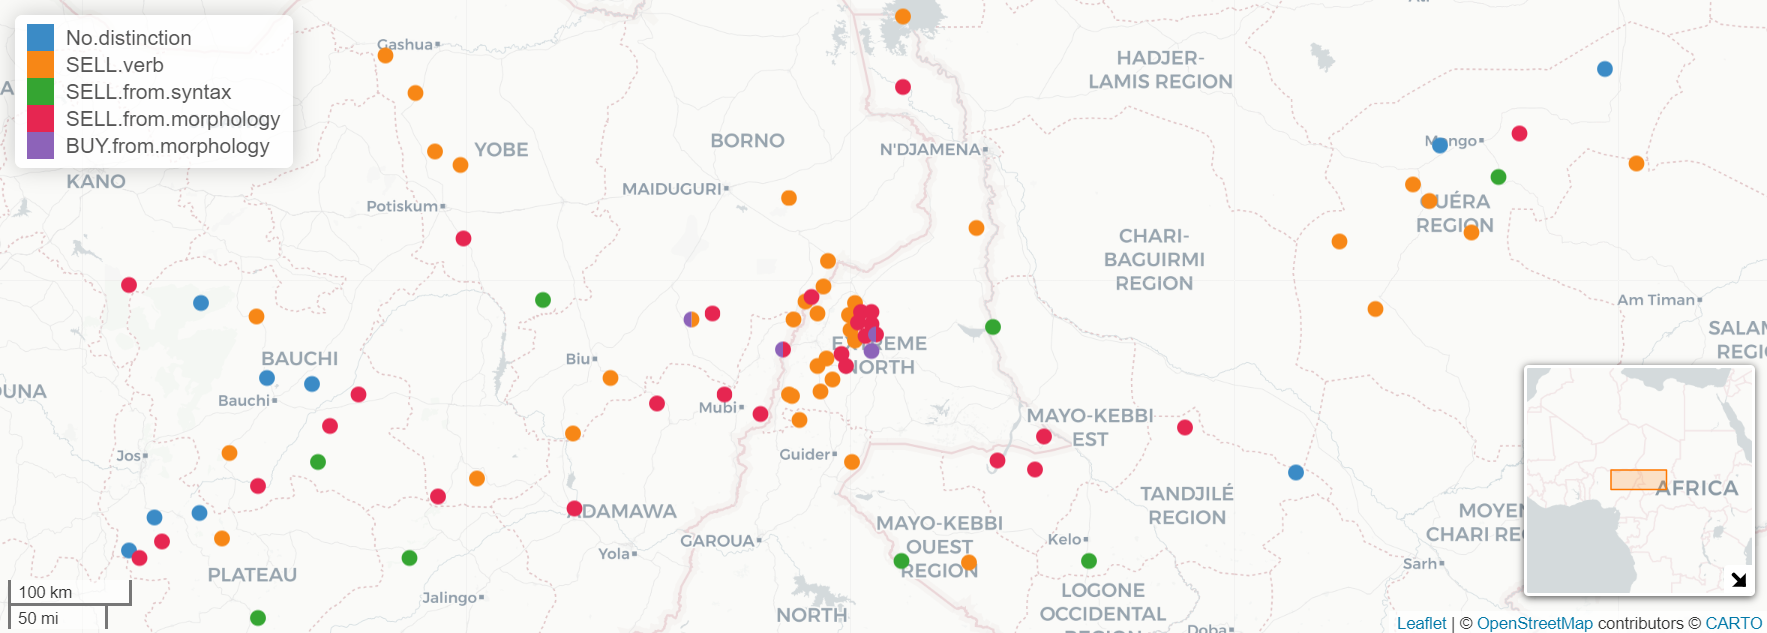
\includegraphics[width=\textwidth]{maps/buy-sell.png}
	\caption{Geographic distribution of forms for distinguishing BUY and SELL} \label{fig:buysell}
\end{sidewaysfigure}

\section{Borrowed verbs or semantic shift}  \label{sec:borrow}

Of the 85 Chadic languages in this sample, 57 have a verb root that expresses BUY. There are two reasons to assume that these BUY verb roots are erstwhile TRADE verb roots which have been restricted in their meaning.\footnote{The number of BUY verb roots may be over-reported relative to TRADE verbs. In multiple descriptions, a verb glossed as `buy' is found to actually be a TRADE verb which can also be used to express SELL. If this is a common oversimplification of how the lexical semantics of these verbs are documented, then it may be the case that more of the BUY verbs will turn out to actually be TRADE verbs.} The first reason is that TRADE and BUY verbs tend to be cognates. The clearest examples of cognates are from 20 Biu-Mandara languages where verb roots that have the consonantal structure \textit{*skm} or similar are frequently found to express TRADE or BUY, as shown in \tabref{tab:cognates}. Reflexes of this form are found in most Biu-Mandara subgroups including all six Dabaic languages, at least six Mofuic languages, six Mandaraic languages and both Hurza languages. Also shown in \tabref{tab:cognates} are likely cognates of the form \textit{*kl} expressing TRADE or BUY in four East Chadic A languages, and the form \textit{*st} for the same meanings in West Chadic A3 languages.  Other likely cognates for any verbs expressing TRADE, BUY or SELL are generally restricted to a single subgroup and only attested in two or three languages.\footnote{As discussed in Chapter \ref{ch:diachrony}, very few lexical items have been reliably reconstructed for Proto-Chadic.}

\begin{table}
	\caption{Verb root cognates expressing TRADE or BUY in Chadic languages}
	\label{tab:cognates}
	\begin{tabular}{llll}
		\lsptoprule
	Branch &	 Language 				&  TRADE &  BUY \\
		\midrule
Biu-Mandara & \hyperref[mbuk]{Mbuko} &   sukom &     \\
Biu-Mandara & \hyperref[vame]{Vamé} &  		  &    səm-  \\
Biu-Mandara & \hyperref[dghw]{Dghwede} &  	  &    skwá  \\
Biu-Mandara & \hyperref[park]{Parkwa} &  		  &    səkw  \\
Biu-Mandara & \hyperref[malg]{Malgwa} &  		  &    shə́kwa  \\
Biu-Mandara & \hyperref[zulg]{Zulgo-Gemzek} &    &    sékém  \\
Biu-Mandara & \hyperref[mada]{Mada} &  	skóm	  &      \\
Biu-Mandara & \hyperref[muya]{Muyang} &  	səkum	  &      \\
Biu-Mandara & \hyperref[wuzl]{Wuzlam} &  	sə̄kə̄m	  &      \\
Biu-Mandara & \hyperref[glav]{Glavda} &  	səgw	  &      \\
Biu-Mandara & \hyperref[molo]{Moloko} &  	skom	  &      \\
Biu-Mandara & \hyperref[mere]{Merey} &  			  &  səkəm    \\
Biu-Mandara & \hyperref[mata]{Matal} &  			  &  sə̀kw    \\
Biu-Mandara & \hyperref[buwa]{Buwal} &  	skām	  &     \\
Biu-Mandara & \hyperref[daba]{Daba} &  	səkəm	  &     \\
Biu-Mandara & \hyperref[gava]{Gavar} &  	 		  &  skəm   \\
Biu-Mandara & \hyperref[mafa]{Mafa} &  	 		  &  súm-   \\
Biu-Mandara & \hyperref[maza]{Mazagway} &  	 		  &  súm-   \\
Biu-Mandara & \hyperref[mbud]{Mbudum} &  	 		  &  sə̀kə̀m   \\
Biu-Mandara & \hyperref[mina]{Mina} &  	 		  &  skəm   \\
\midrule
East A & \hyperref[lele]{Lele} &  	kil 		  &     \\
East A & \hyperref[ndam]{Ndam} &  	kə́lə 		  &     \\
East A & \hyperref[somr]{Somrai} &  	 		  &    kələ  \\
East A & \hyperref[kwan]{Kwang} &  	 		  &    kèle  \\
\midrule
West A3 & \hyperref[mupu]{Mupun} &  	seet 		  &     \\
West A3 & \hyperref[ngas]{Ngas} &  	 		  &    síit  \\
West A3 & \hyperref[goem]{Goemai} &  s'éét	 		  &      \\
		\lspbottomrule
	\end{tabular}
\end{table}

The second reason to assume that BUY verb roots are erstwhile TRADE verb roots is that TRADE and BUY verb roots do not co-occur in the same language. As shown in \tabref{tab:TRADEV}, of the 56 languages with a BUY verb root, none of them have a TRADE verb root. This pattern is naturally explained if the development of BUY verb roots is a semantic restriction of verb roots that previously expressed TRADE.

%data in tab:TRADEV is from python code in file BUYSELL 
\begin{table}
	\caption{Number of languages with a TRADE, BUY or SELL verb roots}
	\label{tab:TRADEV}
	\begin{tabular}{rrrc}
		\lsptoprule
		{} & Has TRADE verb & No TRADE verb  & \% \\
		\midrule
		Has BUY verb 	 & 0 & 56  & \bwpie{0}{56} \\
		Has SELL verb & 6 & 32  & \bwpie{6}{32} \\
		\%  & \bwpie{0}{6} & \bwpie{56}{32} &  \\
		\lspbottomrule
	\end{tabular}
\end{table}

In contrast, as shown in \tabref{tab:TRADEV}, a SELL verb root co-occurs with a TRADE verb root in six languages. Unlike BUY verb roots which are frequently cognates with TRADE, there is just one likely cognate for TRADE and SELL. In the Bura-Marghi subgroup of Biu-Mandara,  we find \hyperref[marg]{Margi} \textit{ɗə̀l} TRADE and \hyperref[huba]{Huba} \textit{ɗəlá} BUY as well as \hyperref[bura]{Bura} \textit{dila} SELL and \hyperref[ciba]{Cibak} \textit{dəl} SELL.

Verb roots that express SELL are regularly described as expressing a range of meanings that include at least one meaning that possibly served as a historically prior meaning that was extended to express SELL. These can be divided into three groups: GIVE/SEND, THROW and LOSE. Four Mandaraic languages use a verb root \textit{vəl} to express SELL. There is evidence that this use is an extension of an older meaning related to transfer of possession. In \hyperref[glav]{Glavda}, the verb also means `give' and in \hyperref[wand]{Wandala} it also means `send'  \citep[155]{frajzyngierGrammarWandala2012}. In other languages, the verb for SELL also means `throw'. This is also the case for SELL verb roots \textit{daw} in \hyperref[mata]{Matal} and \textit{kal} in \hyperref[mere]{Merey}. The closely-related \hyperref[zulg]{Zulgo-Gemzek} verb \textit{kel} `sell' likely has the same history. Two East Chadic languages and one West Chadic language have verbs for SELL which also mean `lose' or `be lost'. This is true for \hyperref[bara]{Barayin} \textit{bito} `be lost' as well as \hyperref[mawa]{Mawa}. In \hyperref[tang]{Tangale} the notion SELL can  be expressed by the verbs \textit{sọgị} `spend, get rid of, lose, sell' and \textit{wayị} `let go, release, sell' \citep[146, 161]{jungraithmayrDictionaryTangaleLanguage1991}.\footnote{In \hyperref[lama]{Lamang}, the verbs \textit{skwa} ‘buy’ and \textit{dzawa} `sell' bear a resemblance to the verb roots \textit{skwa-} `come' and \textit{dza-} `go'. It is unclear whether this is a coincidence or evidence of a historical link.}

It is also possible that forms used to express SELL were borrowed from other languages. This is reported by some \hyperref[buwa]{Buwal} speakers for the verb \textit{bér} `sell' (Melanie Viljoen, personal communication), though it is not clear what the source language would be. This same form is used for SELL in all Dabaic languages. In the closely-related \hyperref[mafa]{Mafa} language, the verb for sell \textit{pə̀r-} `délier, vendre [untie, sell]’ is similar to the Buwal form, but its translation suggests that its use may be derived through a semantic shift. 

In summary, the comparative data provide evidence that verb forms that express TRADE or BUY are likely historical retentions, with BUY verb roots directly derived from erstwhile TRADE verb roots. In contrast, languages that have a verb root dedicated to expressing SELL have likely innovated this form through semantic extension or borrowing. 

\section{Verbal morphology distinguishing SELL}	 \label{sec:SELLmorph}

Besides innovating a new verb root for SELL, the second most common means of distinguishing SELL from TRADE or BUY is to use existing verbal morphology to derive a SELL verb from a TRADE/BUY verb root. This strategy is seen in 30 languages. In 12 of those languages, the morphology used to modify a TRADE/BUY verb root is used elsewhere as a valency-increasing device. In nine languages, the morphology used is used elsewhere as a directional extension. Finally, in nine other languages it is not clear what the function of the verbal morphology is outside of modifying a TRADE/BUY verb to mean SELL. This is either because of the limited data available or because the relevant morpheme is fossilized having lost any other function it previously had in the language. These fossilized forms will not be discussed in this section, as too little is currently known about their likely historical sources. 

\subsection{Valency-increasing morphology distinguishing SELL}	
\largerpage
Among the 12 languages that use a valency-increasing morphological alternation to mark SELL, the relevant morphological form is typically described as a causative. For example, in \hyperref[cuvo]{Cuvok}, the use of the ``causative'' suffix \textit{-dá} with the verb root \textit{husàm} `buy, sell' enforces the meaning `sell' \citep[315]{dadakGrammaireCuvokLangue2021}. This pattern raises the question of whether the concept SELL should be considered a semantically causative predicate (`cause to BUY'). The assumption that SELL is semantically causative is apparent in a description of \hyperref[paaa]{Pa'a} when \citet[189]{skinnerAspectsPaanciGrammar1979} states that, in regard to the verb \textit{kwan} `buy, sell', ``context determines meaning, no ± caus. difference''. Another example of assuming a causative semantic relationship between `buy' and `sell' is Schuh's proposed analysis of the \hyperref[ngam]{Ngamo} verb \textit{bò’ota} `sold' as the causative form of the verb \textit{kàja} `bought' despite the lack of any morphological evidence for this analysis \citep[332]{schuhChadicCornucopia2017}.\footnote{The same assumption is found in an analysis of German \textit{kaufen} `buy' and \textit{verkaufen} `sell'. The \textit{ver-} prefix is not productive and not used in causative contexts, yet \citet[270--271]{kastovskyCausatives1973} classifies the German example as an ``implicit causative''.} 

\largerpage
In \hyperref[haus]{Hausa}, the verb \textit{sàyaa} `buy' in a ``Grade 5'' form becomes \textit{sayar̃} `sell'.  \citet{jaggarHausaGrade52014} cites several scholars as authoritative sources that agree with his conclusion that SELL in Hausa is a semantic causative of BUY.\footnote{If we allow that the seller can be viewed as a causer, then it is equally plausible to view the buyer as a causer. This is precisely what \citet[191]{jackendoffSemanticStructures1990} proposes in giving Lexical Conceptual Structures for English \textit{buy} and \textit{sell} which differ only in which roles are linked to the argument of the outermost CAUSE function which instigates the event. Rather than analyzing \textit{sell} as the causative form of \textit{buy}, both verbs are seen as predicating caused events.} The only clear objection to this analysis is from \citet[398]{newmanEfferentialAliasCausative1983} who judges this analysis to be ``totally inaccurate and without justification.'' One of Newman's arguments is that within the Hausa language \textit{sayar̃} `sell' is not semantically equivalent to `cause to buy' which would be expressed by a periphrastic causative using the verb \textit{saà} `put, cause' \citep[402]{newmanEfferentialAliasCausative1983}.\footnote{The pattern in Hausa can be contrasted with Japhug (Sino-Tibetan) where \citet[17]{jacquesGrammarJaphug2021} uses the label ``inversive'' to refer to the use of a causative form to derive a SELL interpretation from the verb `buy': \textit{sɯ-χtɯ} [buy-\textsc{caus}]. However, this form is said to be translatable as either `cause to buy' or as `sell'.}

A cross-linguistic perspective on Chadic verbal morphology supports Newman's rejection of the analysis of SELL as a causative event. Morphemes that are labeled ``causative'' in Chadic languages often show patterns of use that do not map directly onto a semantic notion of causation as a relationship between a causal and caused event \citep{kulikovCausatives2001} or as the addition of a causer argument to a basic predicate \citep{dixonTypologyCausativesForm2000}. For example, in \hyperref[pero]{Pero}, the suffix \textit{-n} distinguishes \textit{pílù} `buy' from \textit{pílù-n} `sell'. The same suffix \textit{-n} is described as having a causative function in contexts like (\ref{ex:pero100}) where the agent-subject can be seen as causing the patient-object to act (`cause to eat'). 

\ea\label{ex:pero100}
\langinfo{\hyperref[pero]{Pero} verb \textit{cíyyó} `eat' with \textit{-n} suffix}{}{\cite[173]{frajzyngierGrammarPero1989}} \\
\gll cíyyó-n kà míjibà-ì \\
eat.\gl{pl}-\gl{caus} \gl{asoc} stranger-\gl{def} \\
\glt `Feed the strangers.'
\z 

The same \textit{-n} suffix also has a ``benefactive'' function in examples like (\ref{ex:pero101}). 

\ea\label{ex:pero101}
\langinfo{\hyperref[pero]{Pero} verb \textit{cíyyó} `eat' with \textit{-n} suffix}{}{\cite[173]{frajzyngierGrammarPero1989}} \\
\gll n-wálù-n ɓwé \\
and-cook-\gl{ben} gruel \\
\glt `...and the gruel was made for her.'
\z 

The general pattern within Chadic languages is that ``causative affixation is restricted to deriving transitive verbs from verbs that can only be used intransitively in their basic forms'' \citep[287]{schuhChadicCornucopia2017}. Rather than using the specific label \textit{causative} for such multi-functional forms, the more generic label \textit{valency-increasing} is more appropriate.\footnote{However, even this label does not capture all the uses of such morphology, as there is no difference in valency between BUY and SELL.} Given the fact that these valency-increasing morphemes are often found to express meanings other than causative, there is no compelling reason to assume that such morphemes are semantically or morphosyntactically causative in their function when they distinguish SELL from BUY. As \citet[175]{frajzyngierGrammarPero1989} notes in a comparison of Pero and Hausa, ``such an explanation would be purely ad hoc.''

The more likely explanation of why valency-increasing morphology comes to function as a means of distinguishing BUY and SELL stems from its applicative-like function as a marker of a beneficiary or other non-core argument. In the context of a transfer-of-possession event, such marking can refer to a recipient. Marking a non-subject recipient is incompatible with the BUY framing of a commercial transaction, and therefore must express a SELL framing. This underlying logic would explain why this form became conventionalized as a morphological means of making this distinction.\footnote{It remains to be seen whether this explanation has wider validity in other language families where forms labeled \textit{causative} distinguish SELL from BUY. A parallel case can be found in Puyuma (Formosoan) where a beneficiary suffix (glossed \textsc{cv}) is used to express the notion SELL: \textit{trima'-anay} `sell' [trade-\textsc{cv}]'. \citet[156]{kuoArgumentAlternationArgument2015} points out a similar pattern in Formosoan languages, but in those cases the suffix is labeled \textit{causative}: Amis, \textit{pa-qaca} `sell [\textsc{caus}-buy]' and Seediq, \textit{se-m-barig} `sell [\textsc{caus-av}-buy]'. \citet[387]{van1999generalized} mentions the German example alongside Lakhota \textit{ophéthų} `buy' and \textit{iyópheya} `sell' and Tagolog \textit{bili} `buy' and \textit{mag-bili} `sell'.}

Note, however, that not all Chadic languages with valency-increasing morphology use this strategy for distinguishing BUY and SELL. For example, in \hyperref[marg]{Margi} there is a valency-increasing (or causative) verbal suffix \textit{-ani}, but it is the itive directional extension that is used to distinguish SELL from TRADE \citep[119]{hoffmannGrammarMargiLanguage1963}.\footnote{Evidence from Kimaragang (Austronesian) provides further support for the notion that the combination of valency-increasing morphology and BUY verb roots only results in a SELL interpretation when this is lexically specified. There are two Kimaragang verbs for BUY: \textit{boli} and \textit{dagang} \citet[270]{kroegerCaseMarkingKimaragang1988}. While the ``two seem to be perfect synonyms'' the causative verb \textit{po-boli} means `cause to buy' and the causative verb \textit{pa-dagang} means `sell'. The most straightforward explanation of this pattern is that the form \textit{pa-dagang} `sell' is idiomatic.}  

\subsection{Directional extensions distinguishing SELL}	

Other than the valency-increasing (``causative'') forms used to distinguish SELL from TRADE or BUY, there are also at least nine languages that use directional extensions in the same way. Most of these languages use an itive directional extension to distinguish SELL from TRADE or BUY. For example, in \hyperref[wuzl]{Wuzlam}, the verb \textit{sə̄kə̄m} `\textit{acheter} [buy]' with the itive suffix becomes \textit{sə̄kə̄m-arə} `\textit{vendre} [sell]' \citep[162]{colombelLangueOuldemeNordCameroun2005}. In these cases the logic appears to be that the good exchanged is moving away from the seller toward a goal (the recipient).\footnote{The reason that the goods exchanged would be the moving object, and not the money exchanged, is that the exchange of money is lexically entailed and not expressed as a core argument. Therefore, it is the goods that are more likely to be seen as a figure on a path of motion.} \citet[134]{dryerAssociatedMotionDirectionals2021} notes the same pattern in Tamashek (Berber) and treats it as a directional since the ``metaphorical motion of what is bought or sold involves motion towards the buyer/seller or away from them.''

However, there are several reasons that BUY and SELL events should not be treated as motion events. It turns out that it is not always itive direction that is used to mark a SELL interpretation. Three languages use a different directional extension for this purpose. In \hyperref[gude]{Gude}, the verb \textit{ɗərə} `buy, trade' means `sell' when used with an upward/outward suffix: \textit{ɗərəgi} \citep[182]{hoskinsonGrammarDictionaryGude1983}. In \hyperref[psik]{Psikye}, it is the bushward suffix \textit{-mte}, as in (\ref{ex:psik25}).\footnote{The \textit{-mte} suffix in Psikye is also used for itive caused accompanied motion expressions with a `take' verb (Chapter \ref{ch:CAM}).} While the above can all generally be construed as depictions of SELL as an event moving away from a deictic center, the pattern in \hyperref[bole]{Bole} is the opposite. The verb \textit{gójju}  is translated `buy', and the ventive form of the verb, \textit{gòjùttù}, is translated `sell' \citep[36]{gimbaBoleenglishhausaDictionaryAlhaji2004}. As a West Chadic language, Bole has no directional extensions other than ventive. Nonetheless, this one exception demonstrates that there is nothing inherently itive or outward about the semantic relationship between SELL and BUY. A ventive directional extension can equally well distinguish the two concepts. 

Furthermore, if the combination of a BUY verb with itive direction was to be treated compositionally (BUY+ITIVE=SELL), some explanation would be needed for languages which have an itive directional extension and yet do not use it to distinguish BUY and SELL. Two languages, \hyperref[cuvo]{Cuvok} and \hyperref[dghw]{Dghwede}, have an itive extension and yet rather use a valency-increasing form to distinguish SELL. In addition, other directional extensions can be used to mark a BUY predicate. 

\section{Verbal morphology distinguishing BUY}	\label{sec:BUYmorph}

In four Biu-Mandara languages, there is a means of marking a verb meaning TRADE or SELL to instead mean BUY. In two of the languages, the directional extensions used align with the notion that BUY and SELL can be viewed as motion events in which the goods are moving away from or toward the subject. In Giziga, the verb \textit{hìɗík} can mean `trade, sell, buy', but in its ventive form, \textit{hìɗk-ò}, it explicitly means `buy' \citep[150]{shayGrammarGizigaChadic2021}. In \hyperref[molo]{Moloko}, a verb meaning TRADE marked with a ventive directional means BUY, as in (\ref{ex:molo13}). The same verb marked with an itive directional means SELL, as in (\ref{ex:molo14}). 

\ea\label{ex:molo13}
\langinfo{\hyperref[molo]{Moloko} verb \textit{skom} `buy/sell' with ventive marker }{}{\cite[240]{friesenGrammarMoloko2017}} \\
\gll nə̀-sʊkʷɔm=ala awak\\
1\gl{sg}.\gl{pfv}-buy/sell=\gl{vent} goat	\\
\glt `I bought a goat.'	

\ex\label{ex:molo14}
\langinfo{\hyperref[molo]{Moloko} verb \textit{skom} `buy/sell' with itive marker }{}{\cite[240]{friesenGrammarMoloko2017}} \\
\gll nə̀-sʊkʷɔm=alaj awak\\
1\gl{sg}.\gl{pfv}-buy/sell=\gl{itive} goat	\\
\glt `I sold my goat.'
\z

\hyperref[psik]{Psikye} is the one other language with morphological marking of both BUY and SELL meanings. As shown in (\ref{ex:psik25}) in Section \ref{sec:SELLmorph}, the SELL meaning appears with a rare bushward extension on a TRADE verb. The BUY meaning occurs when the same verb is marked with an outward extension, as in (\ref{ex:psik26}). This use of outward motion does not align with the view of BUY as describing goods moving toward the subject. 

\ea\label{ex:psik26}
\langinfo{\hyperref[psik]{Psikye} \textit{pá} `buy/sell' with outward extension}{}{\cite[114]{smithKapsikiLanguage1969}} \\
\gll  pá-ve ɗá wusú \\
buy/sell-\gl{out} 1\gl{sg} thing	\\
\glt `Buy me the thing!'
\z 

In \hyperref[ciba]{Cibak}, it is also the outward suffix that is used to mark a SELL verb root to express BUY, as in (\ref{ex:ciba4}). 

\ea\label{ex:ciba4}
\langinfo{\hyperref[ciba]{Cibak} verb \textit{də̀l} ‘sell’ with outward suffix}{}{\cite[133]{hoffmannZurSpracheCibak1955}} \\
\gll də́l-bà \\
sell-\gl{out} \\
\glt `buy' [German: `\textit{kaufen}']
\z 

In the use of verbal morphology to make a BUY-SELL distinction, there is a a clear asymmetry in the preferred marking of SELL rather than BUY, these four languages show that this is not without exception. Cibak is particularly exceptional in being the only language of the 85 in the data which does not have a verb root that can express BUY or TRADE on its own without a modifier. The data from these four languages also challenge the notion that BUY events are intrinsically linked with motion toward the deictic center. 

\section{Syntactic elements distinguishing SELL}  \label{sec:SELLsyntax}

In seven languages, the grammatical form that distinguishes a SELL interpretation from TRADE or BUY is said to be an independent element that is not part of the verbal morphology, although it is not always clear how consistently these criteria are applied cross-linguistically. In \hyperref[musg]{Musgu}, the adverbial \textit{àdí}, glossed as `\textit{en brousse, hors du village; vers l'extérieur} [in the bush, out of the village; toward the outside]' \citep[71]{tourneuxLexiquePratiqueMunjuk1991}, is used for this purpose. The adverbial is said to be the form that the itive verbal extension \textit{-di} is derived from \citep[133--134]{meyer-bahlburgStudienZurMorphologie1972}. In \hyperref[bidi]{Bidiya}, the adverb used for this function is \textit{ùnda} `\textit{devant} [in front of]' as in \textit{gìdày ùnda} `\textit{vendre} [sell]' \citep[78]{alioLexiqueBidiya1989}. In \hyperref[lele]{Lele}, it is also a bushward (and itive) adverbial that marks SELL events, as in (\ref{ex:lele12}). 

\ea\label{ex:lele12}
\langinfo{\hyperref[lele]{Lele} verb \textit{kil} `buy/sell' with itive adverbial \textit{cáaní}}{}{\cite[161]{frajzyngierGrammarLele2001}} \\
\gll kil	gé	kàmyá	tùmò	cáaní \\
buy/sell	3\gl{pl}	milk	before	to.bush/\gl{itive} \\
\glt `They used to sell milk.'
\z

In \hyperref[tera]{Tera}, the verb \textit{masa} `buy' combines with an itive particle \textit{masa ɓara} `sell' \citep[19]{newmanGrammarTeraTransformational1970}. Rather than grouping this form with the verbal morphology, \citet[314--315]{schuhChadicCornucopia2017} argues that it is better considered an adverbial, based on its syntactic distribution. In \hyperref[guru]{Guruntum}, the relevant form is said to be a preposition \textit{gʷǎi} `away'  \citep[173]{jaggarGuruntumGurdungWest1988}, but there is no further data showing its distribution. 

Causative forms are often described as a verbal suffix or postverbal particle, but in the case of \hyperref[peve]{Pévé} there is a periphrastic causative which is used to distinguish `sell' from `buy/trade', as in (\ref{ex:peve8}).

\ea\label{ex:peve8}
\langinfo{\hyperref[peve]{Pévé} multiword expression for `sell'}{}{\cite[59]{shayGrammarPeve2020}} \\
\gll  na ráʔ tímbì kunə kə́dàn gi tsoɓ rum(-u) \\
1\gl{sg} take calabash \gl{pl} \gl{purp} make purchase 3\gl{sg}(-\textsc{final.vowel}) \\
\glt `I took the calabashes in order to sell them.'
\z

There are also two West Chadic languages where the presence of a particular type of prepositional phrase used with a TRADE or BUY verb root signals a SELL interpretation. Parallel to the use of comitative phrases to express CAM (Chapter \ref{ch:CAM}, Section \ref{sec:dirCAM}), in \hyperref[nyam]{Nyam} a comitative prepositional phrase with the verb \textit{kemd-} `\textit{kaufen} [buy]' becomes `\textit{verkaufen} [sell]', as in (\ref{ex:nyam3}). \citet[127]{andreasGrammatischeBeschreibungNyam2012} describes this as a causative construction.

\ea\label{ex:nyam3}
\langinfo{\hyperref[nyam]{Nyam} verb \textit{kemd} `buy' with comitative prepositional phrase}{}{\cite[127]{andreasGrammatischeBeschreibungNyam2012}} \\
\gll mùdùk kémd-ì yà brédì \\
woman sell-\gl{hab} with bread \\
\glt `The woman usually sells bread.' [German: `\textit{Die Frau verkauft gewöhnlich Brot}.']
\z 

In \hyperref[goem]{Goemai}, the verb \textit{s'éét} `buy/sell' has a SELL interpretation when the item traded is expressed in a comitative prepositional phrase, as in (\ref{ex:goem2}).

\ea\label{ex:goem2}
\langinfo{\hyperref[goem]{Goemai} verb \textit{s'eet} `buy/sell' with comitative prepositional phrase}{}{\cite[217]{hellwigGrammarGoemai2011}} \\
\gll mòe=s'èèt m̠ép góe lá=kè \\
l\gl{pl}.\gl{sbj}=buy/sell(\gl{sg}) 3\gl{pl}.\gl{obj} with \gl{dem}.\gl{sg}.\gl{gen}=chicken \\
\glt `We sold them the little chicken.'
\z 

In these syntactic expressions we see the notions of movement away and causation (or increased valency) used to distinguish SELL from TRADE/BUY, as is commonly found where verbal morphology is used for the same function. There is a possibility that some of these examples are residue resulting from the lack of a clear method for distinguishing morphology and syntax. That ambiguity does not have a significant impact on the overall typology since it is only relevant for a small number of languages, and the semantic patterns of co-expression are similar to those found in verbal extensions. At least some of these cases, however, are quite clear examples of the use of syntactic constructions for this function. The semantic distinction between BUY and SELL can be made in verb roots, through verbal morphology or in a syntactic construction. 

\section{Conclusion}  \label{sec:BUYsummary}

The data from Chadic languages show that there are a variety of ways that languages may choose to distinguish SELL from BUY. A new verb root may be borrowed or the meaning of an existing verb root expressing transfer of possession (e.g., `give', `throw', `lose') may be extended to express SELL. There are two common morphological strategies used. One is to mark a SELL interpretation using valency-increasing morphology that evokes a non-subject recipient. The other is to use a motion metaphor of goods moving away from the subject to mark the SELL framing. These same strategies, valency-increasing and motion metaphor, are also seen in cases where syntactic constructions are employed to express SELL. 

Each of these strategies for expressing SELL are principled in their own right, but the choice of strategy is unpredictable from language to language, even within subgroups of closely related languages. \tabref{tab:SELLsemantics} shows, for each subbranch, how many languages use each of a particular semantic source for developing a means of distinguishing SELL from a TRADE or BUY verb root (including both morphological and syntactic constructions). This diversity confirms that these forms are recent innovations, not inherited from proto-forms.

\begin{table}[H]
	\caption{Number of Chadic languages using each type of semantic source to develop an overt marker for SELL events}
	\label{tab:SELLsemantics}
	\begin{tabular}{lrrrrr} % add l for every additional column or remove as necessary
		\lsptoprule
		Subbranch	      &  ITIVE/BUSH & VENT & OUT & Valency &  Other \\
		\midrule
West Chadic A	& 0 & 1 & 0 & 4 & 4 \\
West Chadic B	& 1 & 1 & 0 & 1 & 0 \\
Biu-Mandara Hurza & 0 & 0 & 0 & 2 & 0 \\
Biu-Mandara North & 2 & 0 & 2 & 3 & 1 \\
Biu-Mandara South & 2 & 0 & 1 & 2 & 0 \\
Masa			  & 0 & 0 & 0 & 1 & 2 \\
East Chadic A	& 1 & 0 & 0 & 2 & 2 \\
East Chadic B	& 0 & 0 & 0 & 1 & 1 \\
		\lspbottomrule
	\end{tabular}
\end{table}

The choice of strategy for distinguishing BUY and SELL cannot be predicted from morphosyntactic properties of each language. These expressions are best viewed as idiomatic expressions. While there are clear metaphorical principles that motivate the use of some forms more than others, the adoption of a particular strategy seems mostly arbitrary. Therefore, complex forms that distinguish BUY and SELL should not be incorporated into a decompositional semantic analysis.

Another pattern that emerges from these data is the striking asymmetry in the overt marking of forms to express SELL. There is substantial evidence of SELL verb roots being innovated, while BUY verb roots appear to be retentions of TRADE verb roots. Morphologically, it is nearly always the SELL form that is marked in comparison to a BUY or TRADE form. Only in four languages is there a BUY form that is overtly marked by verbal morphology, and, in three of those, the marked BUY form exists alongside a marked SELL form. Syntactically, it is also the case that overtly marked forms express SELL, and not BUY.

There are two possible explanations for this pattern. It may be that BUY is less marked (``zero coding'' vs ``overt coding'') because it is the more frequently used expression \citep[43--44]{haspelmathMarkednessWhatReplace2006}. In a cash economy, it is more common to discuss buying than selling. Even farmers or pastoralists who sell their goods would only periodically act as vendors, while they would act as consumers on a much more regular basis. In such a context, the more frequently used meaning may become the default interpretation. 

A second possible explanation for the markedness of SELL is that there is a cognitive bias towards expressing the ``goal'' or recipient argument of transfer of possession events \citep{lakustaStartingEndImportance2005,georgakopoulosFramingDifferenceSources2015}. The BUY interpretation expresses the recipient as subject, thereby matching the speakers' expectation. In contrast, SELL verbs do not express the recipient as a core argument, and so are marked to signal that they go against the default interpretation. 

This comparative study of BUY and SELL forms across Chadic languages provides insights into how to best analyze individual Chadic languages. Morphologically complex forms and syntactic constructions for distinguishing SELL from TRADE or BUY (and, in rare cases, for marking BUY) can be treated as idiosyncratic expressions that were relatively recently adopted. These exceptional forms are the linguistic traces of the socio-economic shift to currency as the dominate means of commercial transaction. 
